\newpage\section{Evaluation of the solution}

To validate the developed prototype, the previously established test cases are verified for the individual requirements. The testing of the test cases provides information about the degree of fulfillment of the requirements. In addition, the fulfillment of requirements that could not be validated by test cases is considered. Subsequently, the usability of the UI of the prototype will be assessed.

\subsection{Prototype validation}
This section looks at the individual test cases from Section \ref{subsec:requirement_validation} and describes both their implementation and the degree to which they have been fulfilled. Furthermore, the fulfillment of requirements that cannot be confirmed by test cases is evaluated. 

\subsubsection*{T1: A welcome and goodbye message is displayed} 

The implementation of this test case can be implemented without further development by the implemented framework. For this purpose, the Information Screen Activity is specified as the first and last step in the experiment data. Furthermore, a corresponding welcome and farewell text is stored in the experiment data. Appendix \ref{appendix:testcases} shows screenshots of the complete fulfillment of this test case.


\begin{figure}[htbp]
    \centering
    \begin{subfigure}[b]{0.3\textwidth}
        \centering
        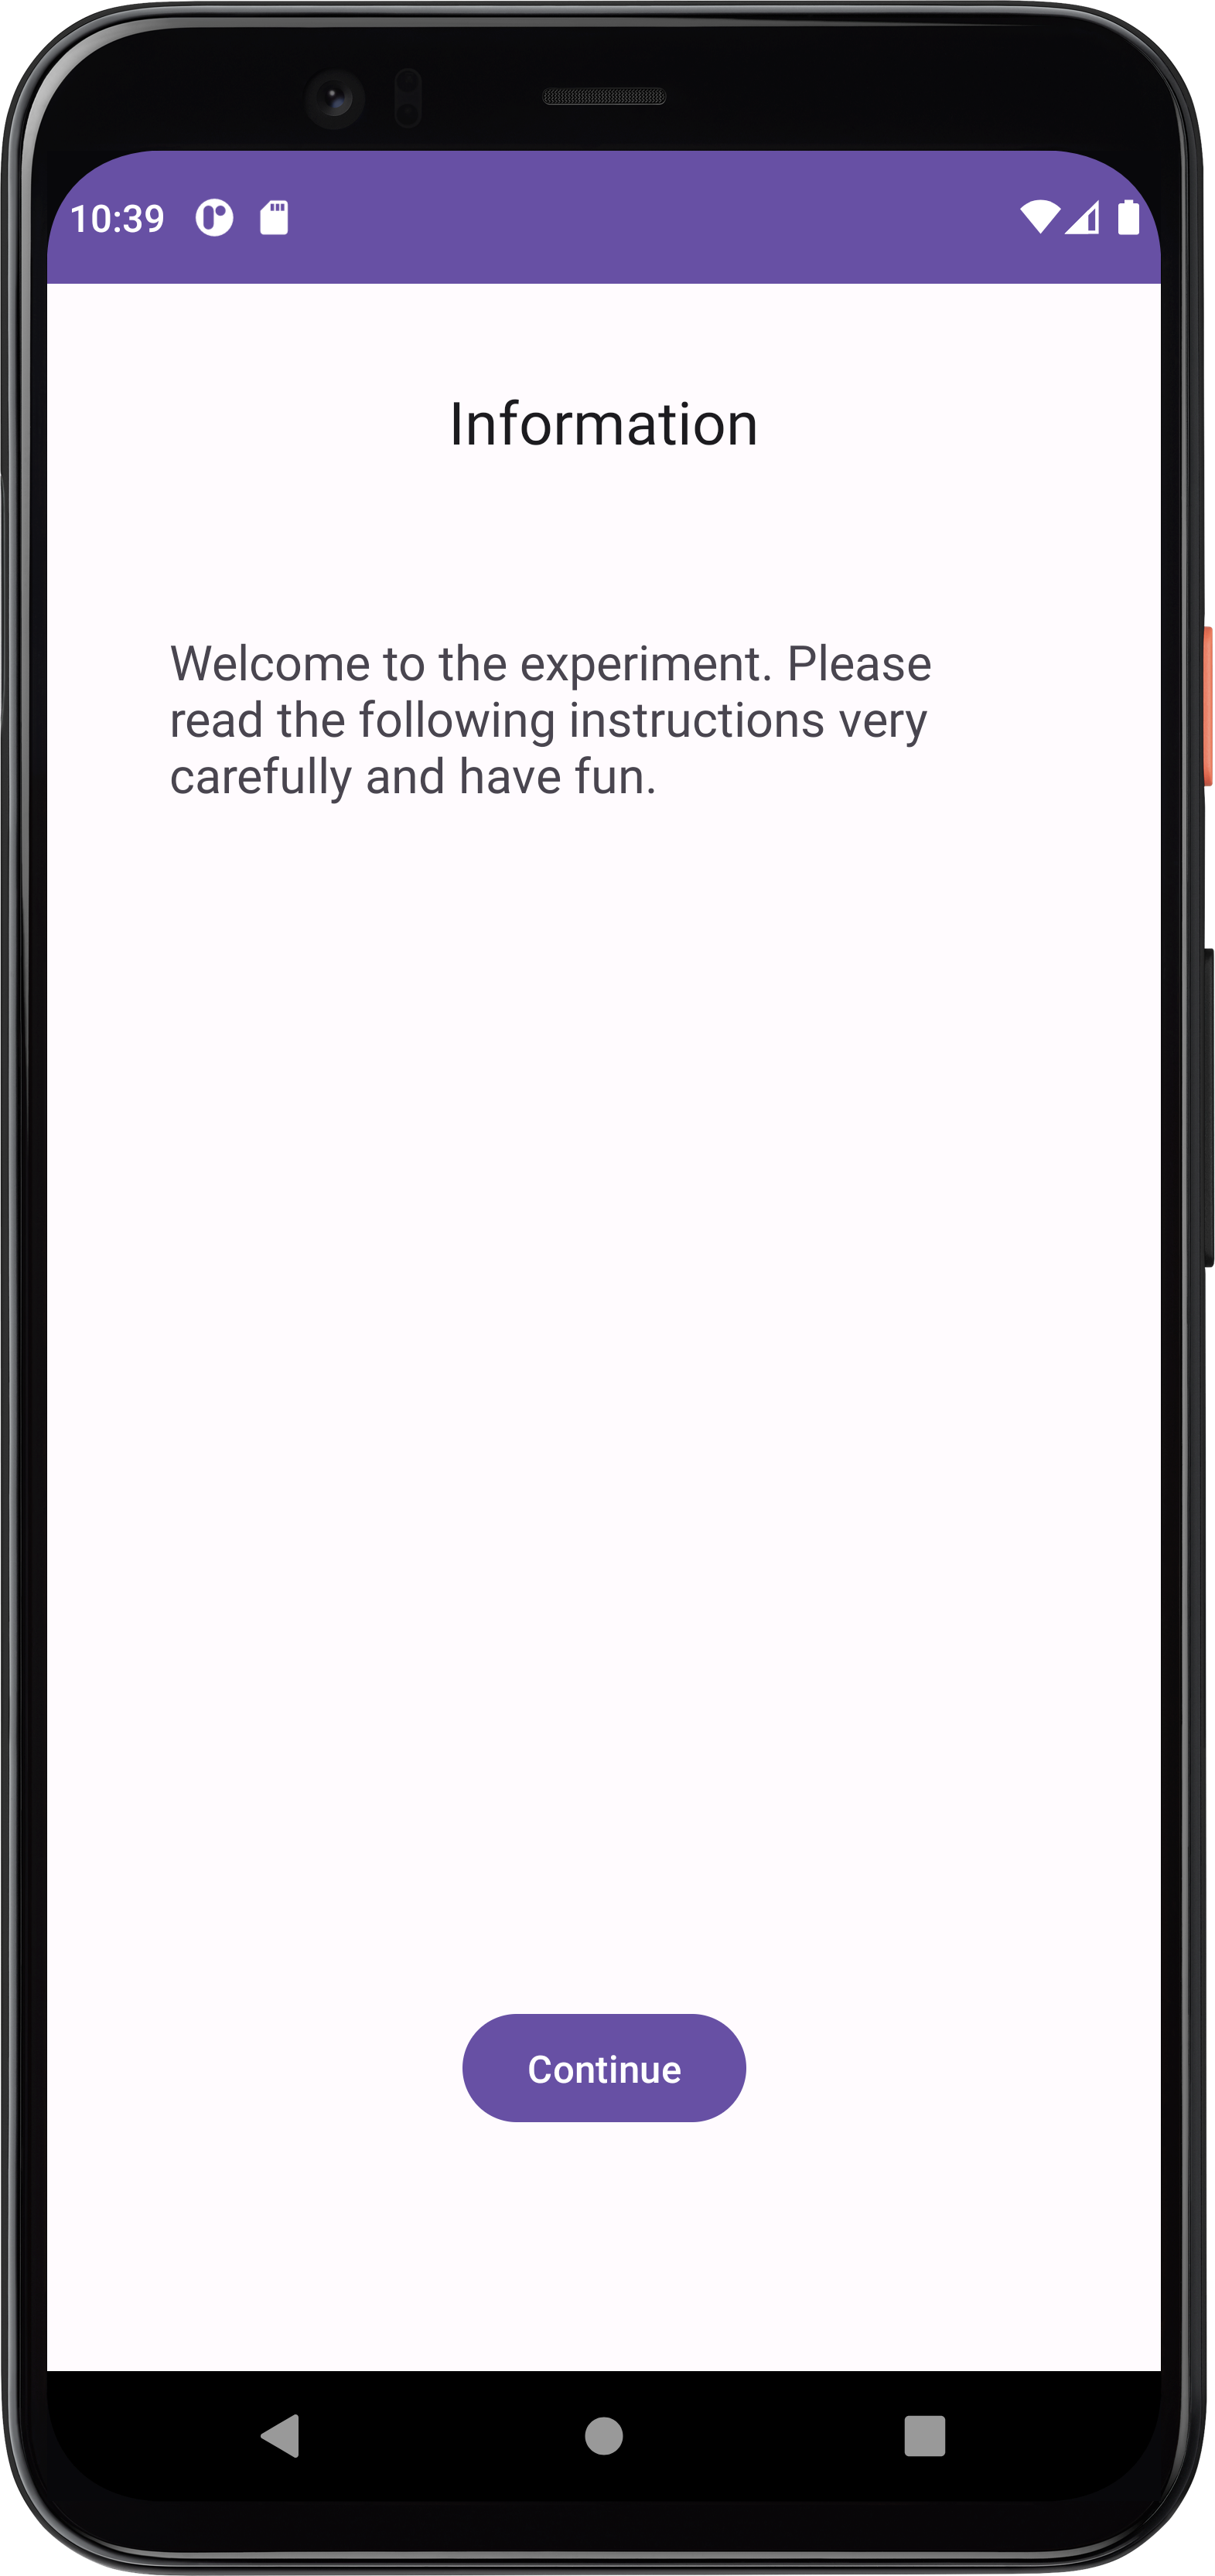
\includegraphics[width=\textwidth]{content/07_evaluation_of_the_solution/Screenshot_StartingScreen.png}
        \caption{Welcome Message}
        \label{subfig:welcomeMessage}
    \end{subfigure}
    \hspace{1cm}
    \begin{subfigure}[b]{0.3\textwidth}
        \centering
        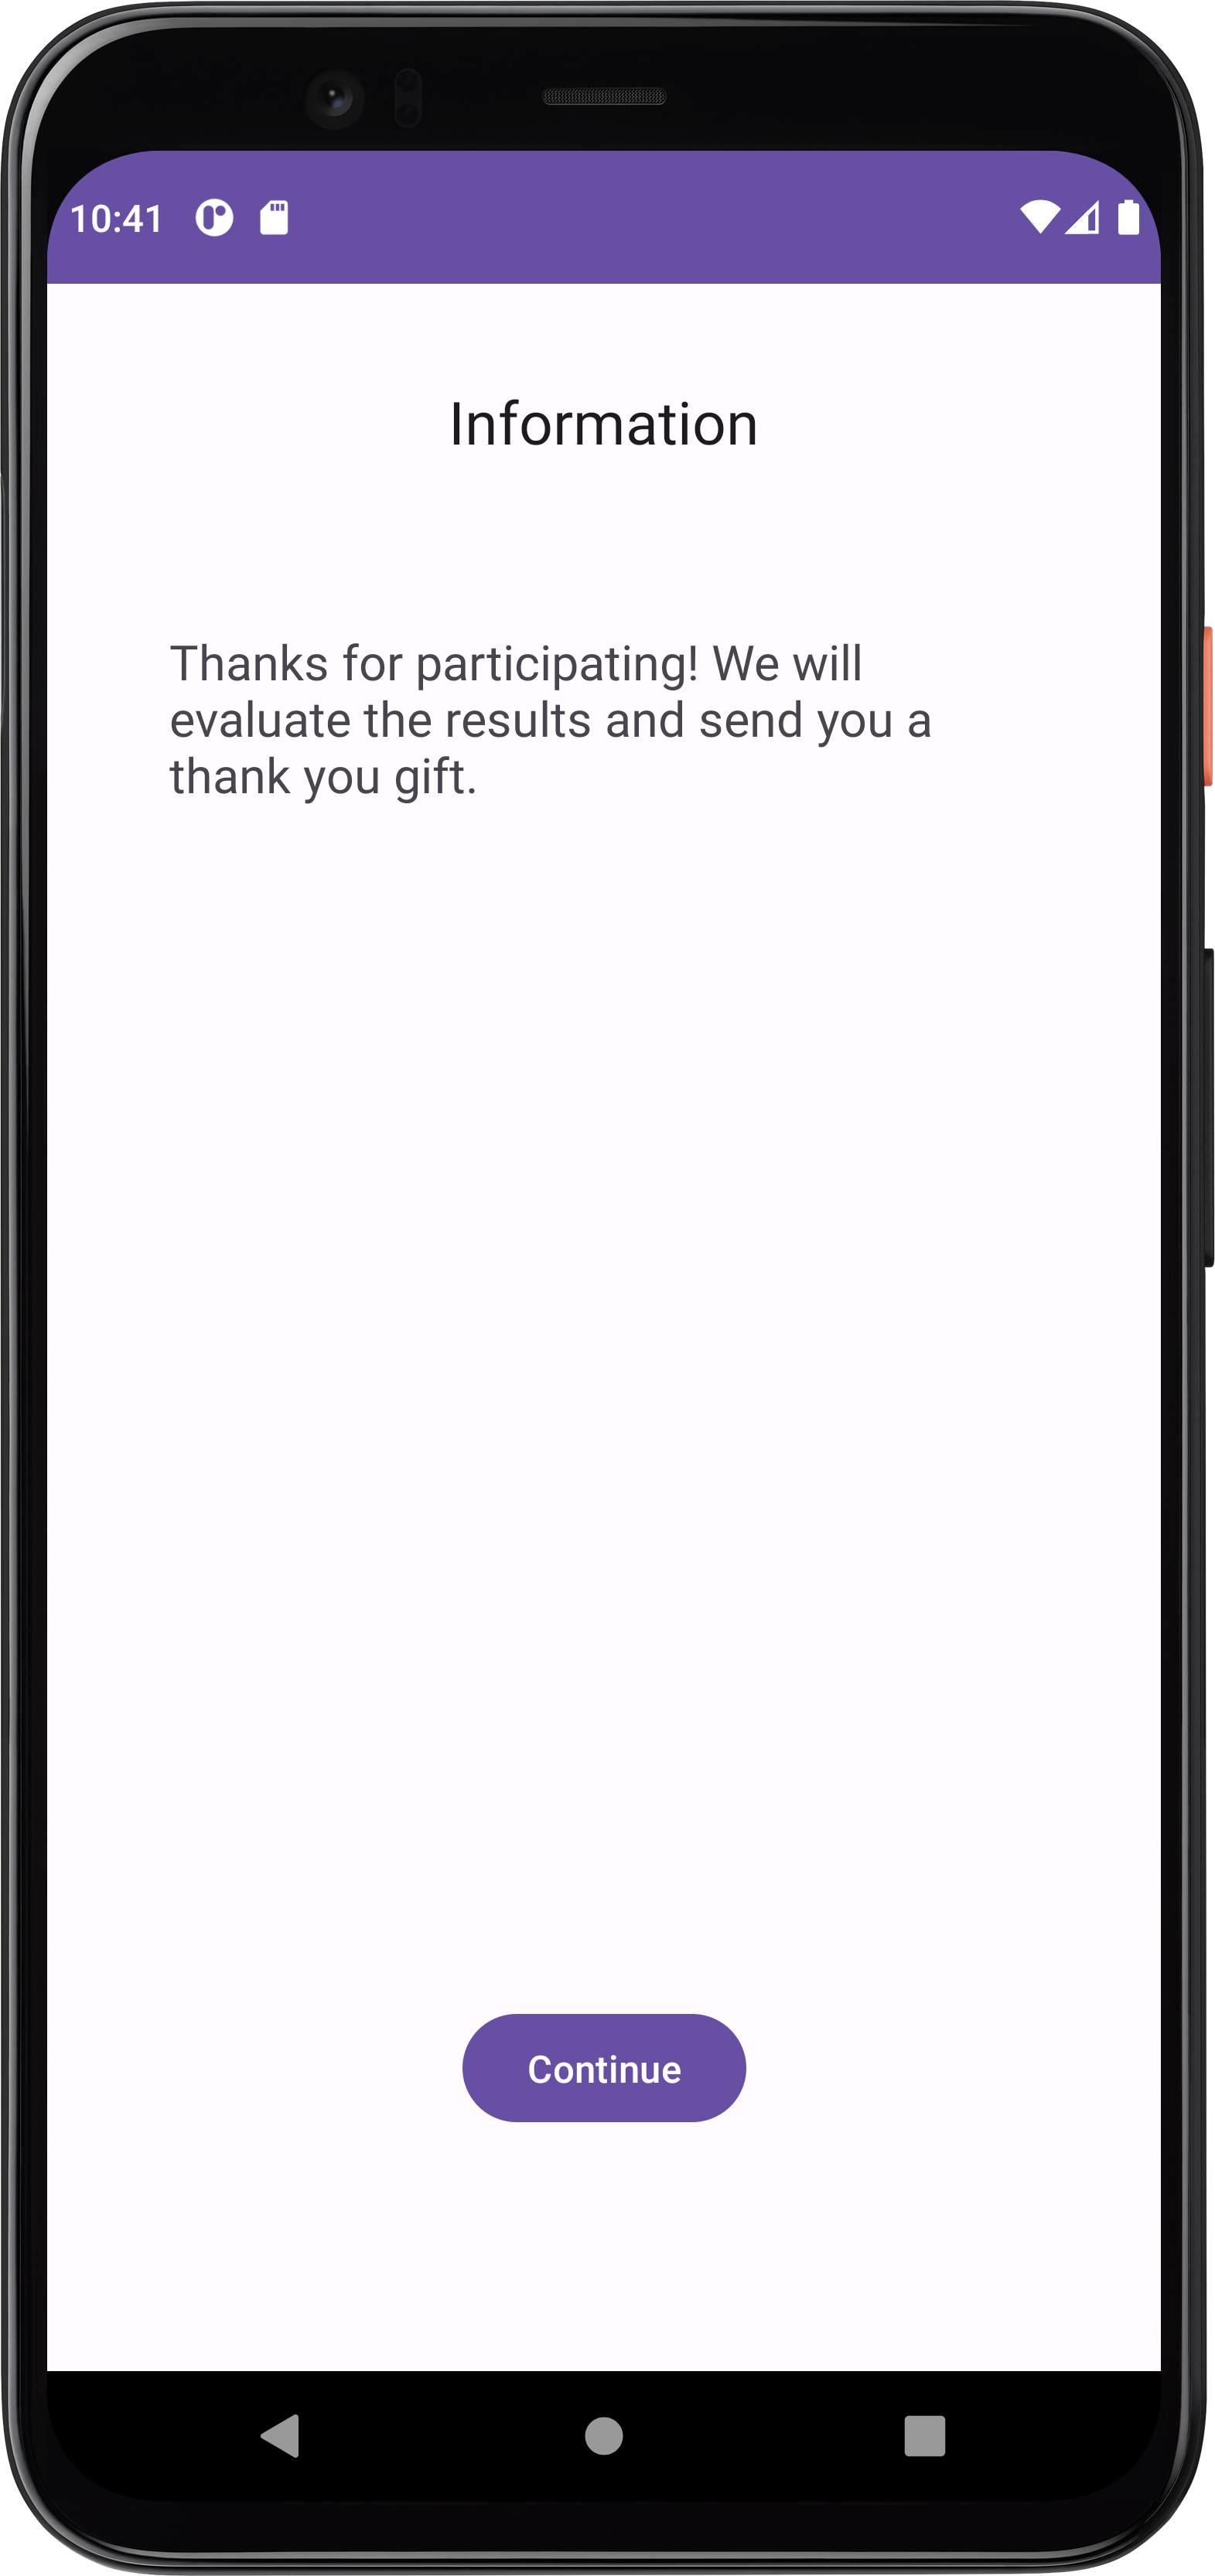
\includegraphics[width=\textwidth]{content/07_evaluation_of_the_solution/Screenshot_GoodbyeMessage.png}
        \caption{Goodbye Message}
        \label{subfig:goodbyeMessage}
    \end{subfigure}
    \caption{User Interface Testcase T1}
    \label{fig:T1}
\end{figure}

\subsubsection*{T2: Participants are prompted to input their age at the beginning and prompted to input how the liked the experiment at the end}


\begin{figure}[htbp]
    \centering
    \begin{subfigure}[b]{0.3\textwidth}
        \centering
        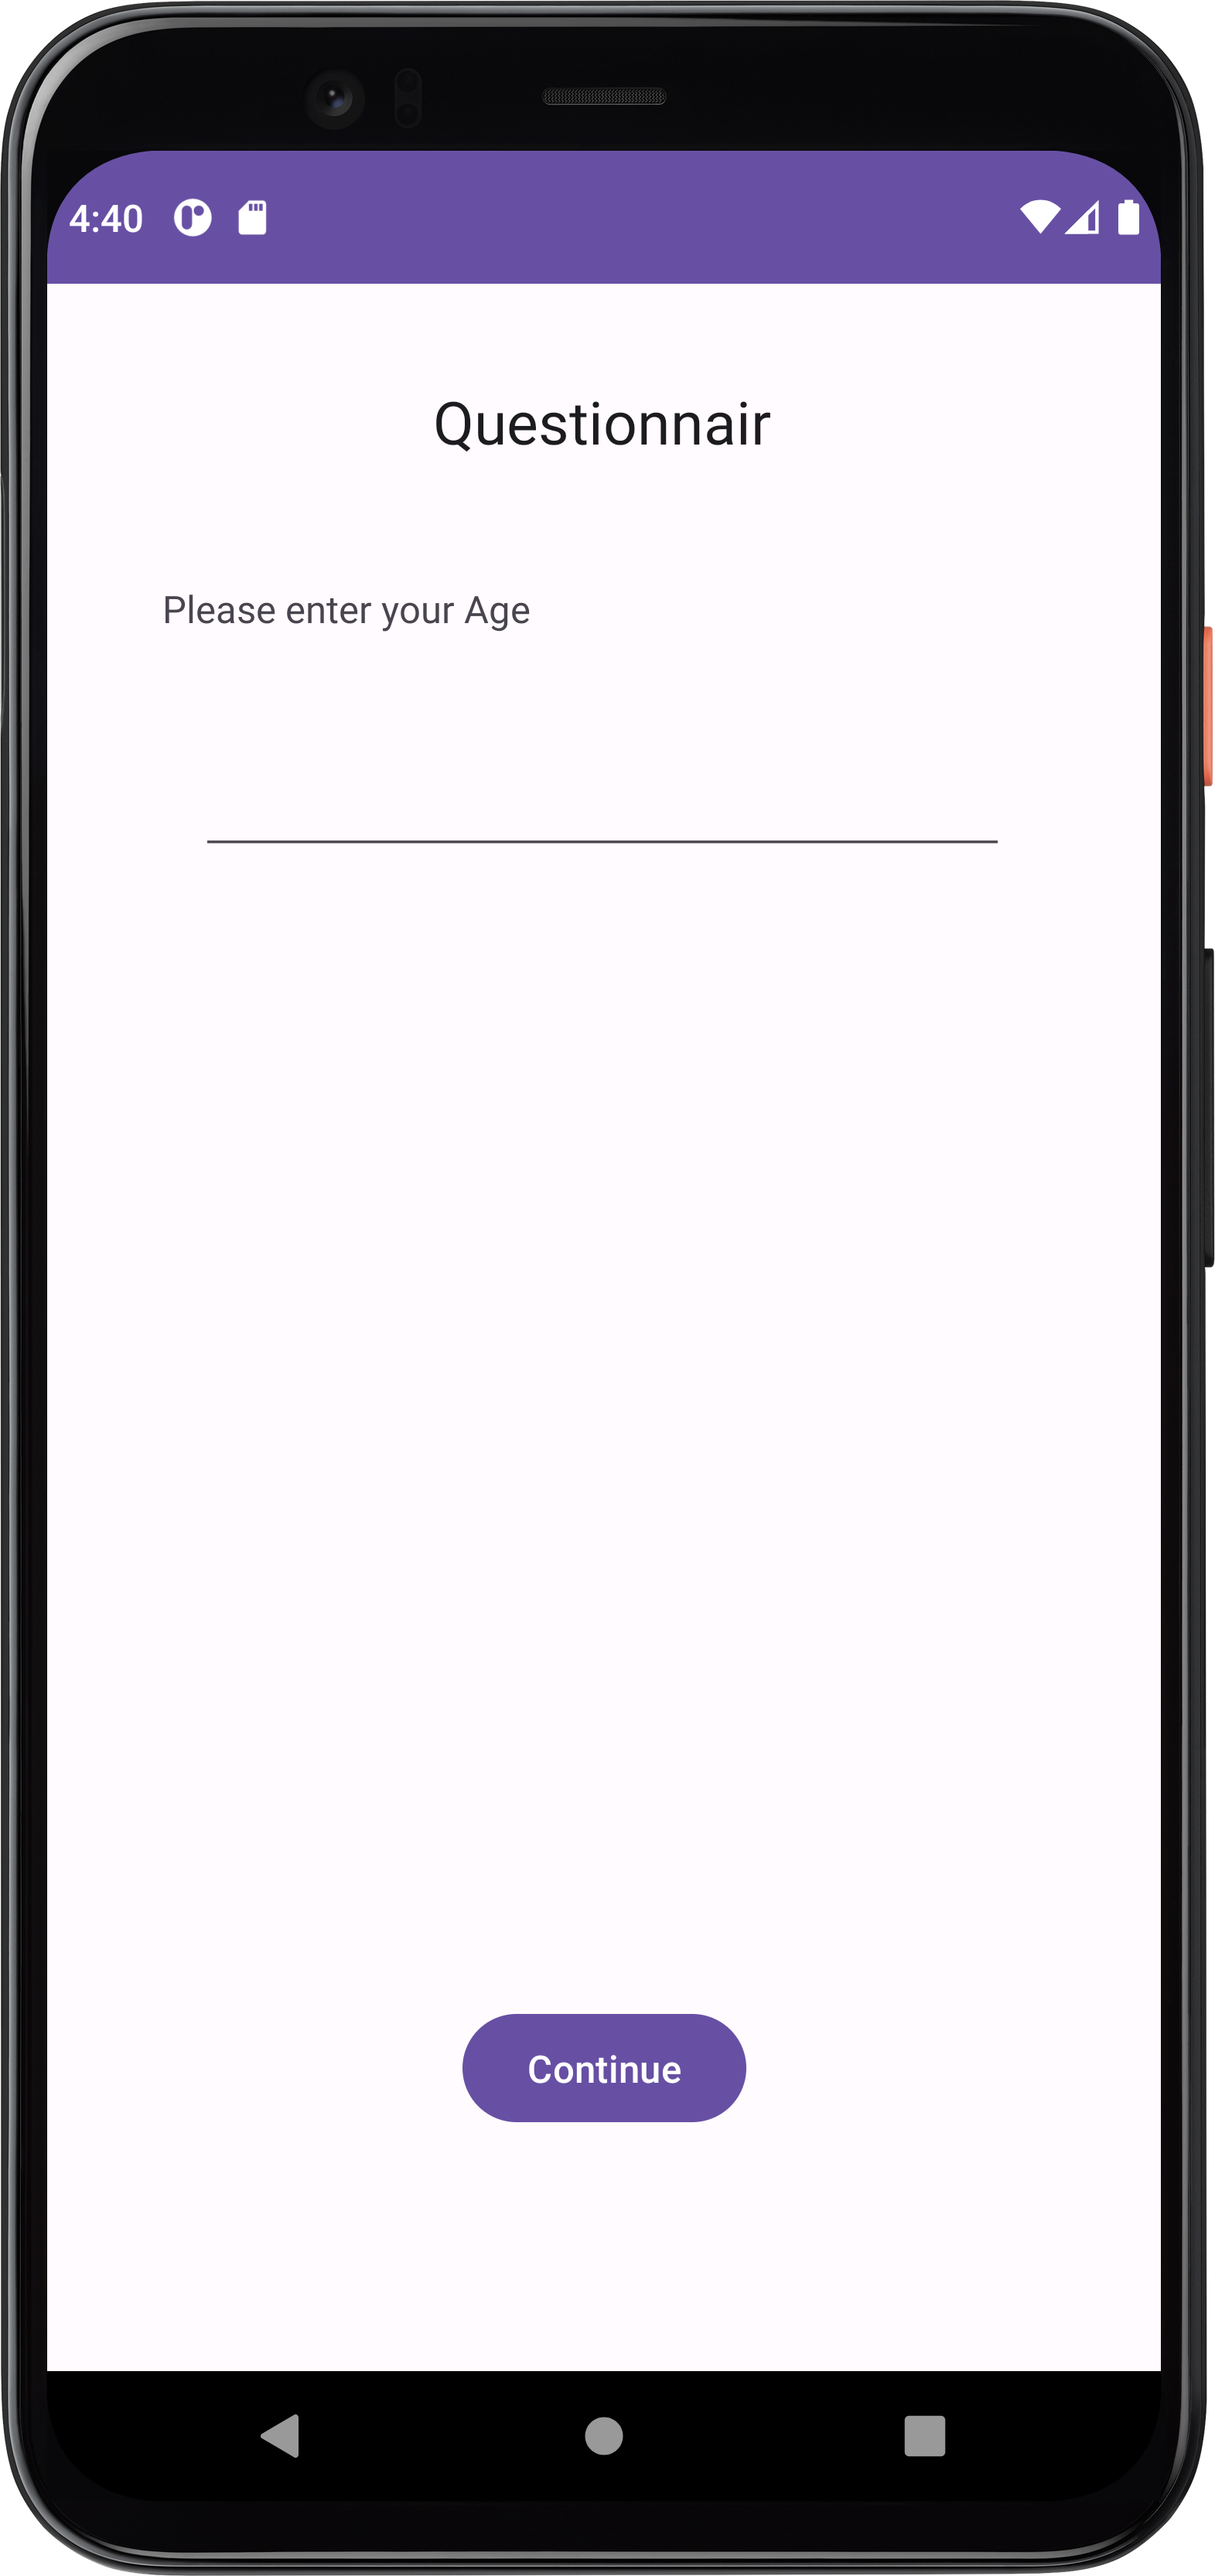
\includegraphics[width=\textwidth]{content/07_evaluation_of_the_solution/Screenshot_T2a.png}
        \caption{Welcome Message}
        \label{subfig:welcomeMessage}
    \end{subfigure}
    \hspace{1cm}
    \begin{subfigure}[b]{0.3\textwidth}
        \centering
        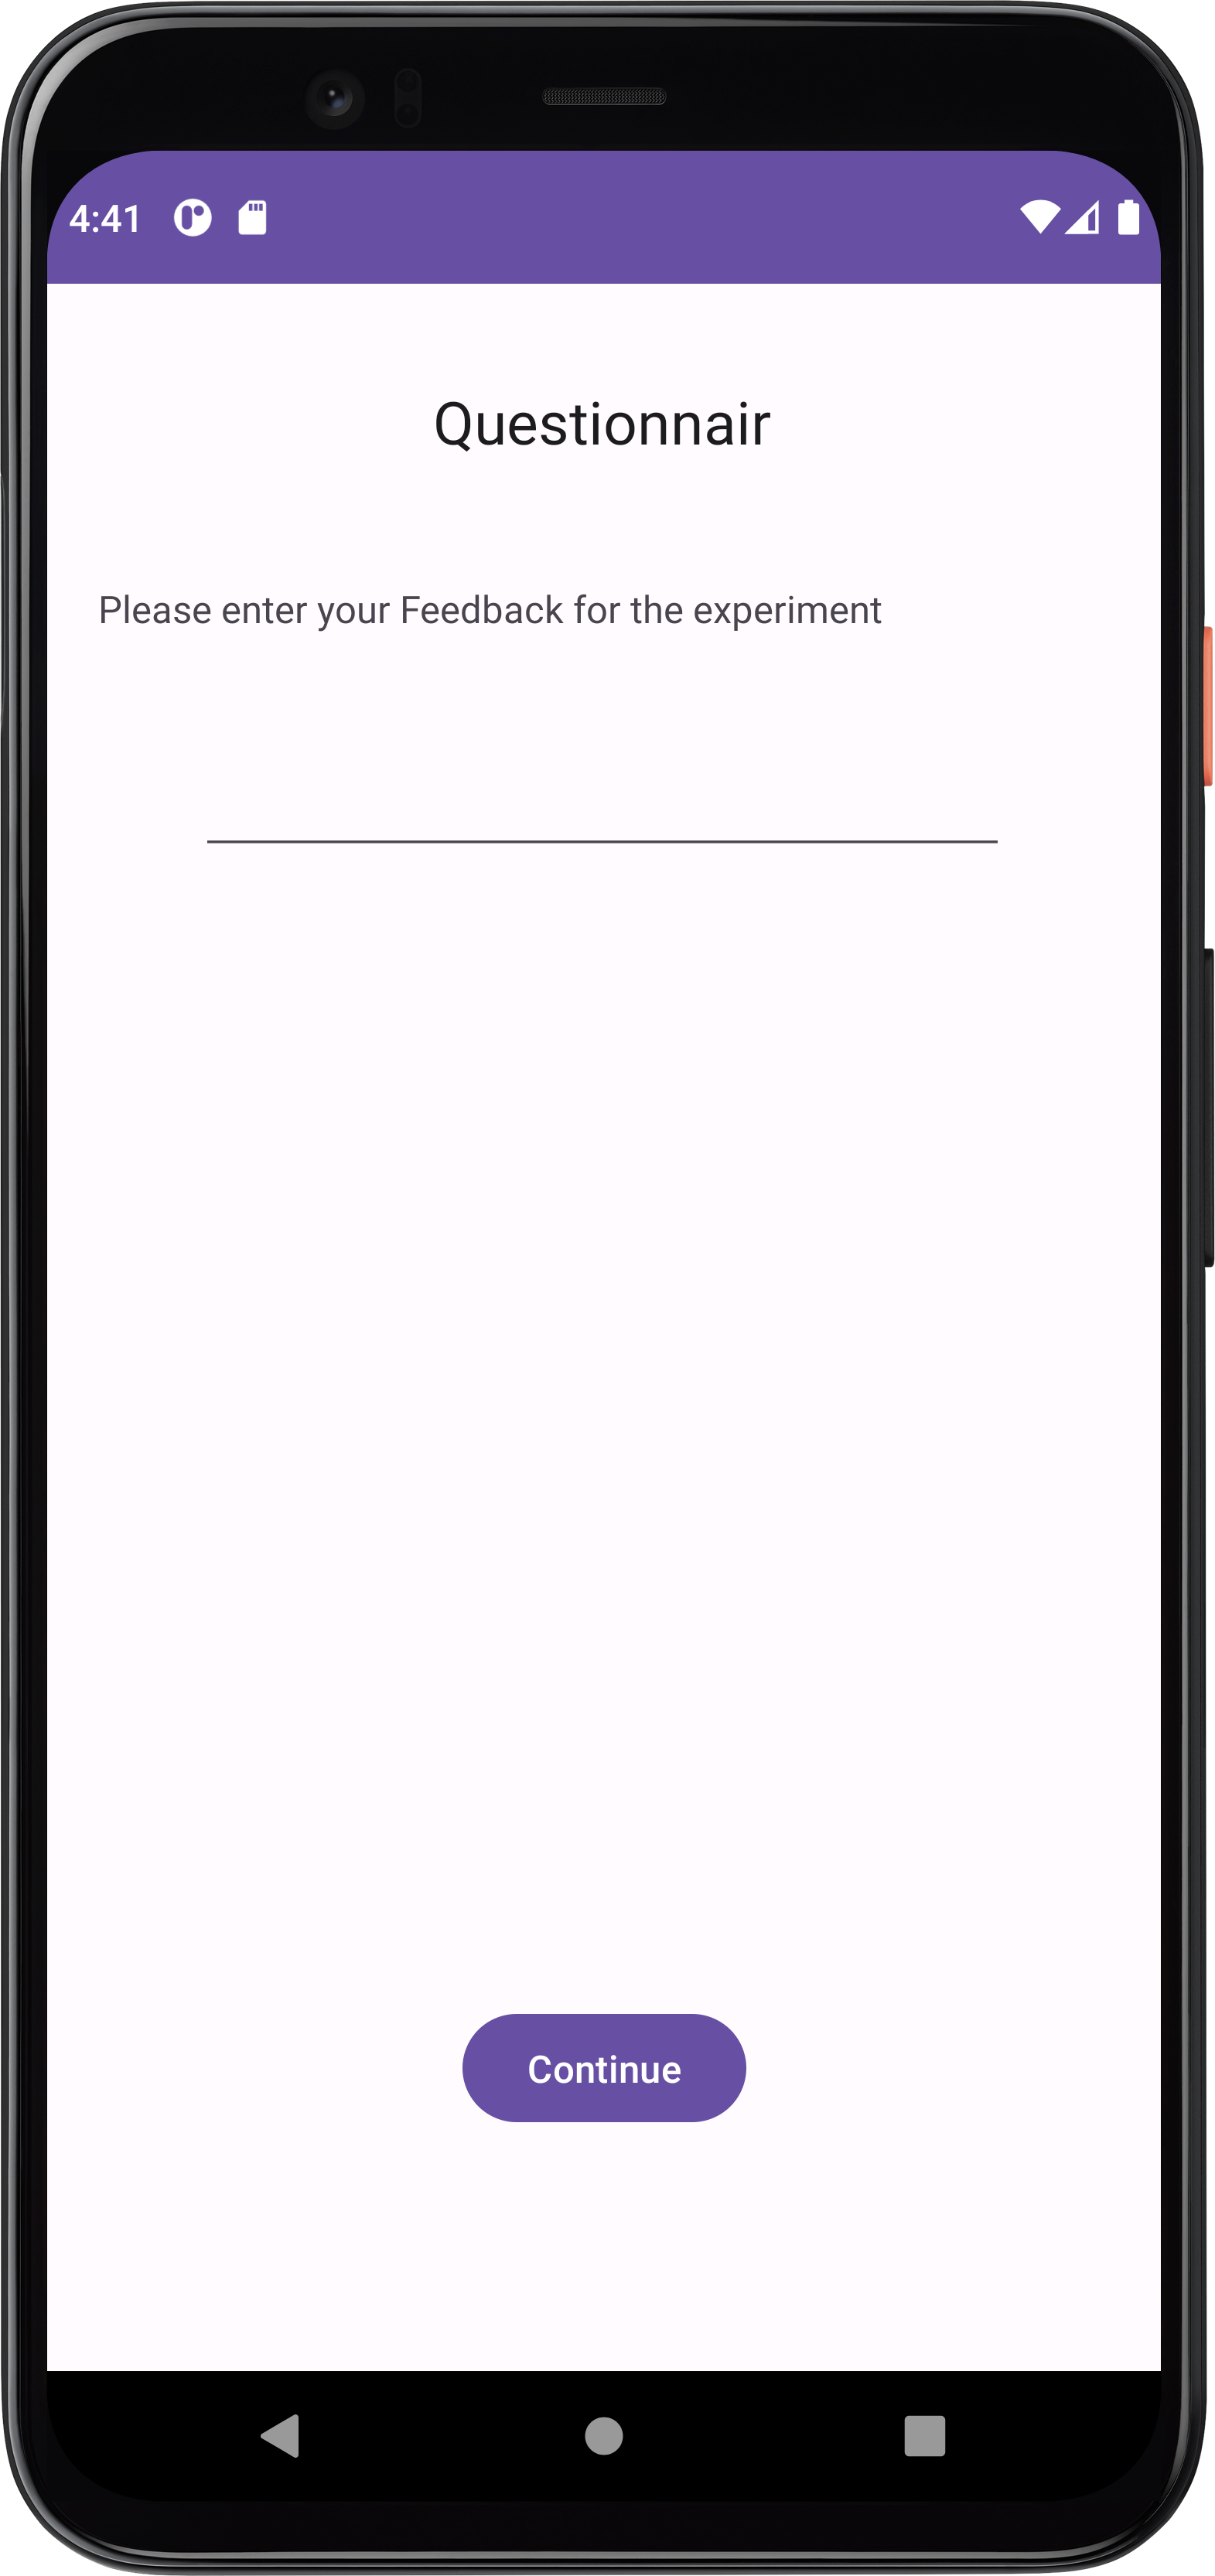
\includegraphics[width=\textwidth]{content/07_evaluation_of_the_solution/Screenshot_T2b.png}
        \caption{Goodbye Message}
        \label{subfig:goodbyeMessage}
    \end{subfigure}
    \caption{User Interface Testcase T1}
    \label{fig:T1}
\end{figure}

\subsubsection*{T3: The information about how long the experiment took is collected}

\begin{lstlisting}[language=java,label=t3a,lineskip={0pt}, caption=Collect time needed to conduct experiment (a), basicstyle=\scriptsize, captionpos=b]
    String currentTime = new SimpleDateFormat("HH:mm:ss", Locale.getDefault()).format(new Date());
    LogMetaDataUseCase.getInstance().setMetaData(currentTime);
\end{lstlisting}

\begin{lstlisting}[language=java,label=t3b,lineskip={0pt}, caption=Collect time needed to conduct experiment (b), basicstyle=\scriptsize, captionpos=b]
    long difference = date1.getTime() - date2.getTime();
    LogMetaDataUseCase.getInstance().setMetaData(difference);
\end{lstlisting}


\subsubsection*{T4: The gender and the weight of the participant is pre-loaded into the experiment from different files. The gender of the participant is deleted}

\subsubsection*{T5: A chess game is added as custom logic}

\subsubsection*{T6: Two groups are created, one of the groups is particularly chosen the other one randomly selected}

\subsubsection*{T7: A chess turn is played by both parties not using the same device}

\subsubsection*{T8 :The results of the experiment are retrieved and displayed in third party software}

\subsubsection*{T9: The experiment is redone a second time and another experimental setup is implemented}

\subsubsection*{T10: The experiment is conducted on different devices}

\subsubsection*{T11: During the experiment the current state of the chess board is exported to the conducter of the experiment}

\subsubsection*{Remaining requirements}



%\subsection{Prototype Testing}



\subsection{App Performance and Usability}
